\let\negmedspace\undefined
\let\negthickspace\undefined
\documentclass[journal]{IEEEtran}
\usepackage[a5paper, margin=10mm, onecolumn]{geometry}
\usepackage{lmodern} % Ensure lmodern is loaded for pdflatex
\usepackage{tfrupee} % Include tfrupee package

\setlength{\headheight}{1cm} % Set the height of the header box
\setlength{\headsep}{0mm}     % Set the distance between the header box and the top of the text

\usepackage{gvv-book}
\usepackage{gvv}
\usepackage{cite}
\usepackage{amsmath,amssymb,amsfonts,amsthm}
\usepackage{algorithmic}
\usepackage{graphicx}
\usepackage{textcomp}
\usepackage{xcolor}
\usepackage{txfonts}
\usepackage{listings}
\usepackage{enumitem}
\usepackage{mathtools}
\usepackage{gensymb}
\usepackage{comment}
\usepackage[breaklinks=true]{hyperref}
\usepackage{tkz-euclide} 
\usepackage{listings}
\def\inputGnumericTable{}                                 
\usepackage[latin1]{inputenc}                                
\usepackage{color}                                            
\usepackage{array}                                            
\usepackage{longtable}                                       
\usepackage{calc}                                             
\usepackage{multirow}                                         
\usepackage{hhline}                                           
\usepackage{ifthen}                                           
\usepackage{lscape}

\begin{document}

\bibliographystyle{IEEEtran}
\vspace{3cm}

\title{6.6.15}
\author{EE24BTECH11052 - Rongali Charan}
% \maketitle
% \newpage
% \bigskip
{\let\newpage\relax\maketitle}

\renewcommand{\thefigure}{\theenumi}
\renewcommand{\thetable}{\theenumi}
\setlength{\intextsep}{10pt} % Space between text and floats

\textbf{Question:}
\newline
Show that the altitude of the right circular cone of maximum volume that can be inscribed in a sphere of radius $R$ is $\frac{4R}{3}$.
\newline
\textbf{Theoretical Solution:}

Let $R$ be the radius of the sphere and $h$ be the height (altitude) of the inscribed cone. Let $x$ be the radius of the base of the cone.

By considering a cross-section of the sphere and the inscribed cone, we can relate $x$, $h$, and $R$ using the Pythagorean theorem.  The center of the sphere lies on the axis of the cone.  If we let the distance from the sphere's center to the base of the cone be $y$, then $h = R + y$. Also, $x^2 + y^2 = R^2$.  Therefore, $y = h-R$, and substituting gives:

\begin{align}
x^2 + (h-R)^2 &= R^2 \\
x^2 + h^2 - 2hR + R^2 &= R^2 \\
x^2 &= 2hR - h^2
\end{align}

The volume $V$ of the cone is given by:

\begin{align}
V &= \frac{1}{3} \pi x^2 h \\
V &= \frac{1}{3} \pi (2hR - h^2) h \\
	V &= \frac{1}{3} \pi (2Rh^2 - h^3)   \implies \sbrak{ Cost Function}
\end{align}

To maximize the volume, we take the derivative of $V$ with respect to $h$ and set it equal to zero:

\begin{align}
\frac{dV}{dh} &= \frac{1}{3} \pi (4Rh - 3h^2) \\
0 &= 4Rh - 3h^2 \\
0 &= h(4R - 3h)
\end{align}

Since $h$ cannot be zero, we have:

\begin{align}
4R - 3h &= 0 \\
h &= \frac{4R}{3}
\end{align}

To confirm that this is a maximum, we can take the second derivative of $V$ with respect to $h$:

\begin{align}
\frac{d^2V}{dh^2} &= \frac{1}{3} \pi (4R - 6h)
\end{align}

Substituting $h = \frac{4R}{3}$:

\begin{align}
\frac{d^2V}{dh^2} &= \frac{1}{3} \pi (4R - 6(\frac{4R}{3})) \\
&= \frac{1}{3} \pi (4R - 8R) \\
&= -\frac{4\pi R}{3}
\end{align}

Since the second derivative is negative, this confirms that $h = \frac{4R}{3}$ corresponds to a maximum volume.

\textbf{Computational Solution (Gradient Ascent):}

We can also find the maximum volume using the Gradient Ascent method. The iterative update rule is:

\begin{align}
h_{n+1} &= h_n + \alpha \frac{dV}{dh}\Big|_{h=h_n}
\end{align}

where $\alpha$ is the learning rate.  In our case:

\begin{align}
h_{n+1} &= h_n + \alpha \frac{\pi}{3} (4Rh_n - 3h_n^2)
\end{align}

Taking $R=1$ (without loss of generality, as the result scales linearly with R), and:

\begin{align}
\alpha &= 0.0001 \\
h_0 &= 0.5
\end{align}

After a few iterations, the value of $h$ will converge to approximately $\frac{4}{3} \approx 1.333$.
\begin{figure}[h]
\centering
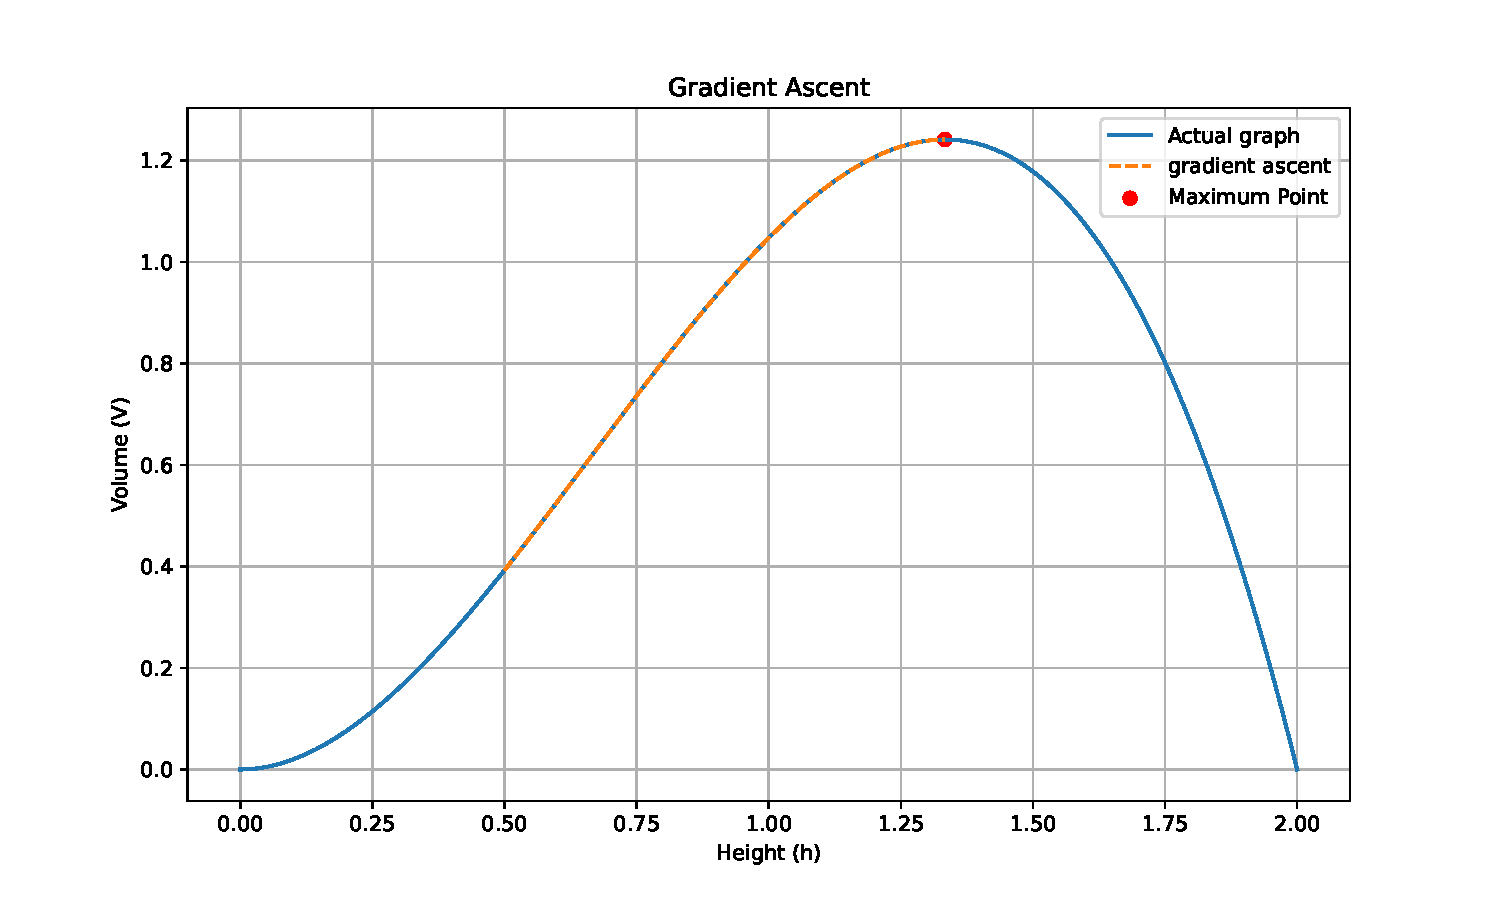
\includegraphics[width=\columnwidth]{figs/plot.pdf}
\label{fig:Plot1} 
\end{figure}
\end{document}

